% DEFINE DOCUMENT PROPERTIES
\documentclass[twocolumn]{article} % Set to two columns
\title{\textbf{LaTeX Basics}}
\author{personam-solis}
\date{August 29, 2026}

\usepackage[margin=0.75in]{geometry} % Set margin to 1 inch
\usepackage{fancyhdr}   % Required for custom headers/footers
\usepackage[T1]{fontenc} % Required to use emphasis and italic
\usepackage{graphicx}   % Required for adding graphics
\usepackage[labelfont=bf]{caption} % Make 'Figure N' bold
\usepackage{cuted}   % Allows breaking columns mid-page
\usepackage{caption} % Allows \captionof outside of a float environment

\pagestyle{fancy}       % Turn on fancy style
\fancyhf{}              % Clear default headers and footers

% Set the header: Center = Document Name
\fancyhead[C]{LaTeX Basics}

% Set the footer: Left = Creator, Center = page number, Right = render date
\fancyfoot[L]{\small Creator: personam-solis}
\fancyfoot[C]{\textbf{\thepage}}   % Bold
\fancyfoot[R]{\small Compiled on: \today} % Also Small Text


% START ACTUAL DOCUMENT (With title)
\begin{document}

% Cancel two column to properly draw title and abstract
\twocolumn[
  \begin{@twocolumnfalse}
    \maketitle % typeset the title (overrides style)
    \begin{abstract}
      This document helps in figuring out how to make nice, and pretty looking LaTeX typeset PDF's. Since i want most documents to have a 'professional' feel, the abstract will take up the full width of the page, while the rest of the body will use the 'two-column' format. Keeping in mind that if there are figures or graphs that need a lengthy explination, it needs to span the whole page in a smaller font size.
    \end{abstract}
    \vspace{2em} % Adds space before the columns start
  \end{@twocolumnfalse}
]

% Empty line after the abstract
\vspace{\baselineskip}

% \section{INTRODUCTION} % You can also use section/subsection and it will also auto-number
\begin{center}
\textbf{1. INTRODUCTION}
\end{center}
The distinct dietary requirements of the Eclectus parrot stem from its unique digestive system. This species features a "longer and more sensitive digestive tract" engineered to "super-absorb the nutrients from their diet".
 This remarkable efficiency, while beneficial in their natural habitat, renders them \emph{"particularly susceptible to hypervitaminosis,"} a condition arising from an excessive accumulation of vitamins.
 This characteristic presents a challenge for caretakers, as what \textit{might be a beneficial nutrient level} for other parrots could become toxic for an Eclectus.
\footnote{This is a footnote that can contain details or a citation}

\begin{figure}[htbp] % Standard envionment keeps it in one column
    % For the figure specifiers:
    %  h - HERE  Place the figure exactly where it is written in the source code, 
    %       right in the middle of the text flow.
    %  t - TOP Place the figure at the top of the current page (or the next page).
    %  b - BOTTOM Place the figure at the bottom of the page.
    %  p - PAGE Place the figure on a dedicated page that contains only figures and tables
    % With all of them together: Try to put it right here. If it doesn't fit, 
    %  put it at the top of a page. If that looks bad, put it at the bottom. 
    %  If all else fails, put it on its own page.
  \centering
  % sizing to \linewidth fills the single column
  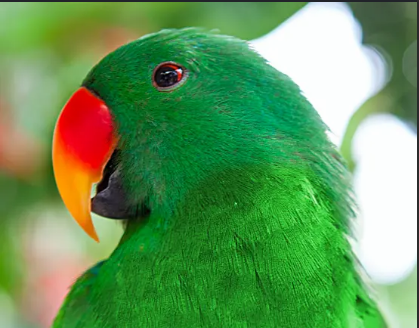
\includegraphics[width=\linewidth]{resources/eclectus.png}
  \caption{This is the caption of the figure. and as you can see it keeps the format
  of the page while also ensuring that the figure is in the column and fills it}
  \label{fig:eclec1} % Create a unique key (anchor) for the figure
\end{figure}

\vspace{\baselineskip}

Ordered
\begin{enumerate}
  \item This is an example
  \item Of an ordered
  \item list of
  \item things
\end{enumerate}

\vspace{\baselineskip}

Unordered
\begin{itemize}
  \item This is an example
  \item of an unordered
  \item list of
  \item things
\end{itemize}

\vspace{\baselineskip}

The consequences of nutritional imbalances in Eclectus parrots are significant and varied.
Hypervitaminosis, for instance, can manifest as "plaque buildup, discolored feathers, toe-tapping, and heightened sensitivities".
In severe instances, these discomforts may even lead to "self-destructive habits like feather plucking or mutilation" as the bird attempts to cope. Such manifestations underscore the critical importance of a precisely balanced diet that respects their unique metabolic pathways.

Furthermore, Eclectus parrots require a "much lower-fat diet" compared to many other parrot species. High-fat diets are associated with "unwanted weight gain" and have been observed to cause "cholesterol deposits in the bird's eye". Their natural diet in the wild, described as a "feast fit for herbivorous royalty – forest fruits, nuts, seeds, and blossoms" , inherently emphasizes fresh, nutrient-rich plant-based foods, which are naturally lower in fat than many commercial seed mixes. This distinction highlights that their evolutionary diet is fundamentally different from that of typical "seed-eating" parrots.

Despite their susceptibility to hypervitaminosis, Eclectus parrots exhibit a "higher requirement for [Vitamin A] compared to other parrots". A deficiency in this vital nutrient can lead to serious health complications, including "respiratory infections, poor feather quality, and weakened immune function". This seemingly contradictory need for high Vitamin A while being prone to hypervitaminosis is resolved by understanding the source of the vitamin. Eclectus parrots thrive when they obtain their Vitamin A from beta-carotene-rich foods, which are precursors that the bird's body converts into active Vitamin A as needed. This mechanism allows them to


\begin{strip} % breaks the figure placement out of the environment
  \centering
  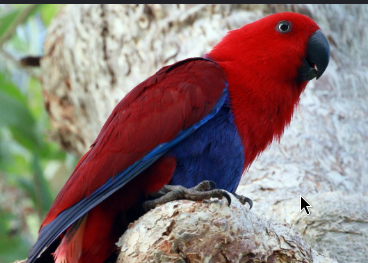
\includegraphics[width=0.8\textwidth]{resources/eclectus2.png}
  % Used \captionof{figure}{...} so it works perfectly inside the strip environment
  \captionof{figure}{This is the caption of the figure. and as you can see it breaks the format of the double column page}
  \label{fig:eclec2}
\end{strip}


The rest of the text resumes from where it left off. and as you can see it resumes from formatting it with two columns.
The consequences of nutritional imbalances in Eclectus parrots are significant and varied.
Hypervitaminosis, for instance, can manifest as "plaque buildup, discolored feathers, toe-tapping, and heightened sensitivities".
In severe instances, these discomforts may even lead to "self-destructive habits like feather plucking or mutilation" as the bird attempts to cope. Such manifestations underscore the critical importance of a precisely balanced diet that respects their unique metabolic pathways.

Furthermore, Eclectus parrots require a "much lower-fat diet" compared to many other parrot species. High-fat diets are associated with "unwanted weight gain" and have been observed to cause "cholesterol deposits in the bird's eye". Their natural diet in the wild, described as a "feast fit for herbivorous royalty – forest fruits, nuts, seeds, and blossoms" , inherently emphasizes fresh, nutrient-rich plant-based foods, which are naturally lower in fat than many commercial seed mixes. This distinction highlights that their evolutionary diet is fundamentally different from that of typical "seed-eating" parrots.

Despite their susceptibility to hypervitaminosis, Eclectus parrots exhibit a "higher requirement for [Vitamin A] compared to other parrots". A deficiency in this vital nutrient can lead to serious health complications, including "respiratory infections, poor feather quality, and weakened immune function". This seemingly contradictory need for high Vitamin A while being prone to hypervitaminosis is resolved by understanding the source of the vitamin. Eclectus parrots thrive when they obtain their Vitamin A from beta-carotene-rich foods, which are precursors that the bird's body converts into active Vitamin A as needed. This mechanism allows them to

\newpage

\begin{center}
\textbf{2. MATH}
\end{center}

A sentence with inline mathematics: $y = mx + c$.
A second sentence with inline mathematics: $5^{2}=3^{2}+4^{2}$.

As you can see above, inline math mode is marked using a pair of dollar symbols ($...$). It is also possible to use the notation \( ... \). Simple expressions are entered without any special markup, and you’ll see that the math is spaced out nicely and has letters in italic.

Inline math mode restricts vertical size of the expression so that as far as possible the formula does not disturb the linespacing of the paragraph.

Note that all mathematics should be marked up as math, even if it is a single character use ... $2$ ... not ... 2 ... otherwise, for example, when you need a negative number and need math to get a minus sign the ... $-2$ ...

USE detokenize to make a string literal!!
use \detokenize{\begin{equation}} to make equations easier and to auto number them

% Also make it look bigger
{\Large
\begin{equation}
F \geq \frac{\Delta I \cdot \Delta t}{\Delta V}
\end{equation}
}

\end{document}
